\documentclass[xcolor=dvipsnames]{beamer} % dvipsnames gives more built-in colors
\mode<presentation>

\usetheme{Boadilla}

\definecolor{GWdarkblue}{HTML}{033C5A}

\usecolortheme[named=GWdarkblue]{structure}

% Sets the font
\usepackage[defaultfam,tabular,lining]{montserrat}
\setbeamerfont{title}{shape=\scshape}
\setbeamerfont{frametitle}{shape=\scshape}
%Remove "Figure" from captions
\setbeamertemplate{caption}{\raggedright\insertcaption\par}

\usepackage{graphicx}
\usepackage{tabularx}
\usepackage{hyperref}

\title[Sampling]{Sampling}
\author[SMPA 2152]{Data Analysis for Journalism and Political Communication (Fall 2024)}
\date{Prof. Bell}

\begin{document}

%%%%%%%%%%%%%%%%%%%%%%%%%%%%%%%%%%%%%%%%%%%%%%%%%%%%%%%%%%%%%%%%%%
\frame{
\titlepage
}

%%%%%%%%%%%%%%%%%%%%%%%%%%%%%%%%%%%%%%%%%%%%%%%%%%%%%%%%%%%%%%%%%%
\frame{\frametitle{1970 Vietnam War Draft}
\only<1>{
    \centering
    \href{https://www.youtube.com/watch?v=OkJH6sapQMA}{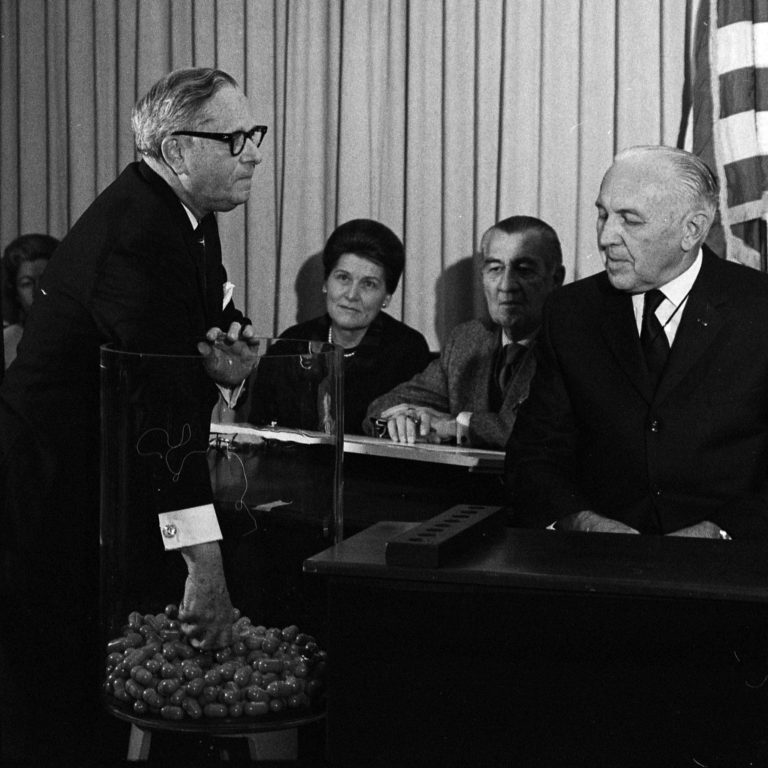
\includegraphics[height = .8\textheight]{lottery_image.jpg}}
}
\only<2>{
    \centering
    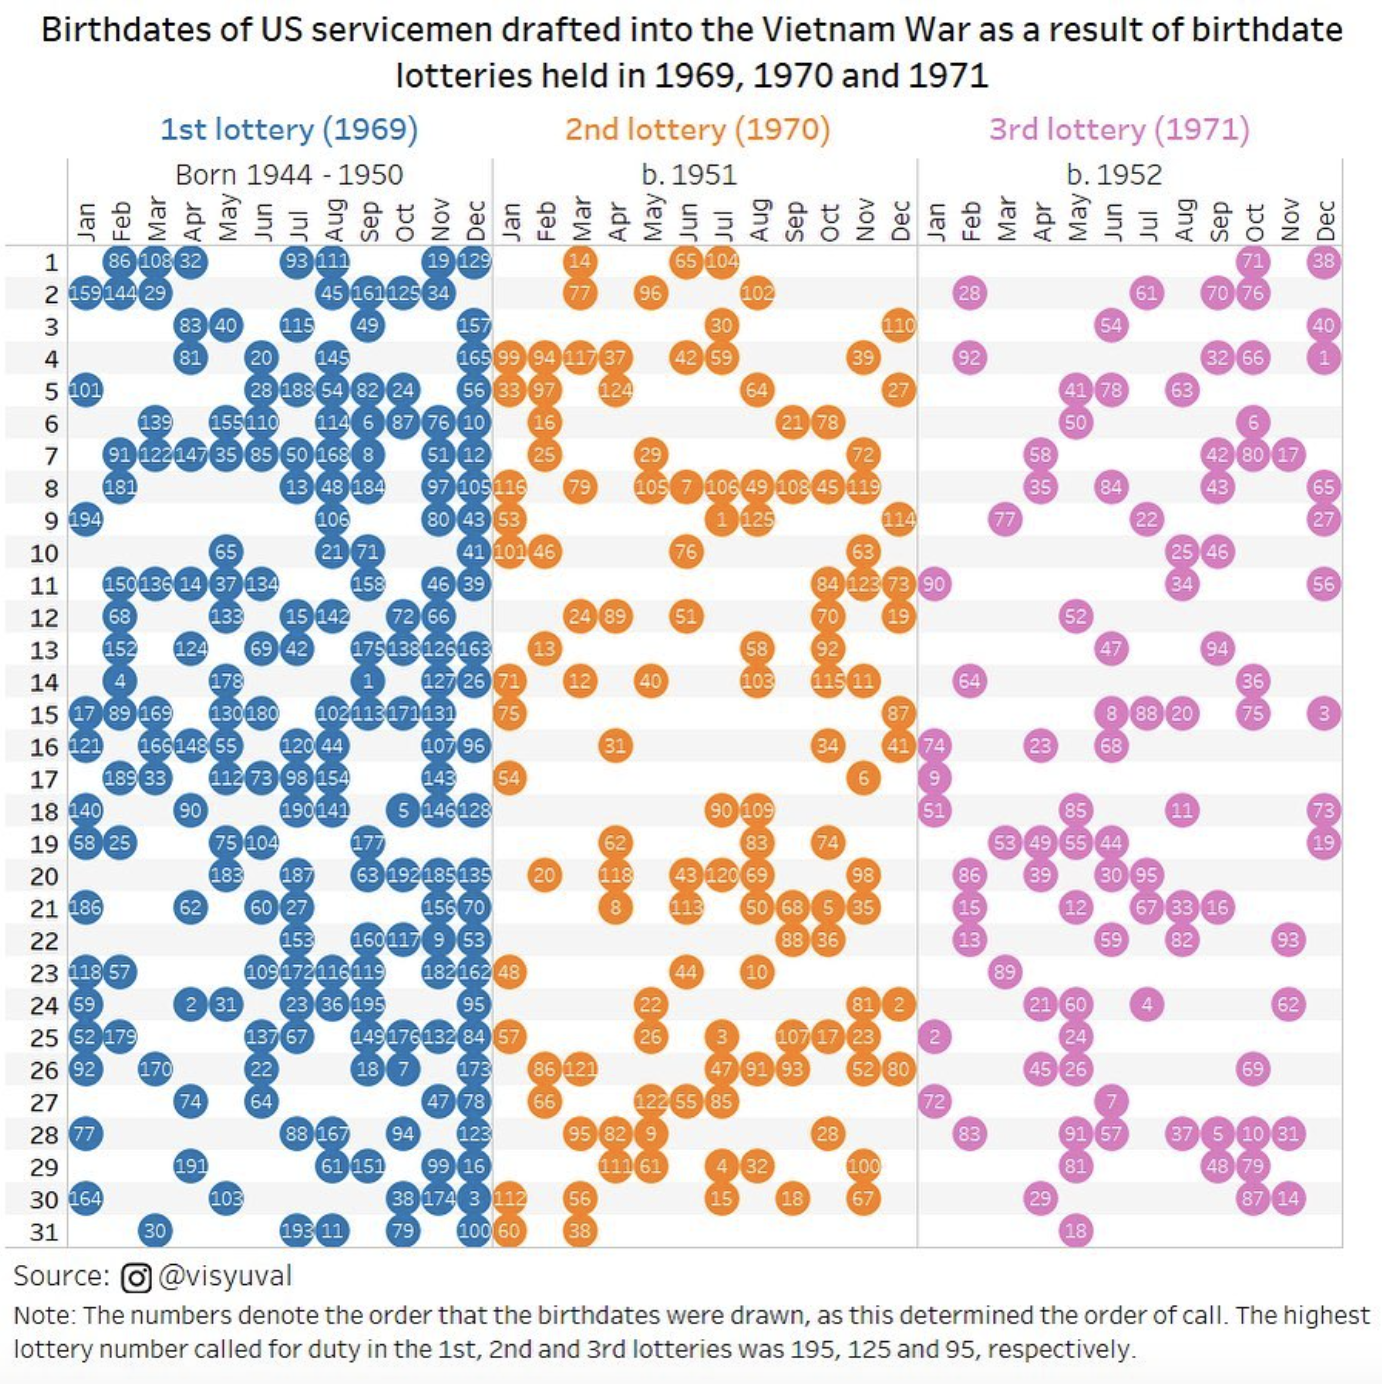
\includegraphics[height = .8\textheight]{vietnam_lottery_data.png}
}
}

%%%%%%%%%%%%%%%%%%%%%%%%%%%%%%%%%%%%%%%%%%%%%%%%%%%%%%%%%%%%%%%%%%
\frame{\frametitle{Definitions}
\begin{itemize}[<+->]
    \item The group we are interested in studying is known as the \textbf{population}
    \item Often, we are not able to count every unit in the population, so we take a \textbf{sample}
    \item Our best guess about the population based on our sample is the \textbf{estimate}
\end{itemize}
}

%%%%%%%%%%%%%%%%%%%%%%%%%%%%%%%%%%%%%%%%%%%%%%%%%%%%%%%%%%%%%%%%%%
\frame{\frametitle{Sampling}

\begin{itemize}[<+->]
    \item There are many ways to derive an estimate from a sample, but recall that ``garbage in = garbage out'': no amount of statistical wizardry can compensate for bad data
    \item The key to any data analysis project is a quality sample, which is determined by two elements:
    \begin{enumerate}
        \item A \textbf{random sample} of the population
        \item<5> The \textbf{sample size} is sufficiently large
    \end{enumerate}
\end{itemize}

\only<4>{\begin{block}{Definition}
    The probability of any given unit being drawn from the population is uniform (the same)
\end{block}}
}

%%%%%%%%%%%%%%%%%%%%%%%%%%%%%%%%%%%%%%%%%%%%%%%%%%%%%%%%%%%%%%%%%%
\frame{
\Large
In-class exercise
}

%%%%%%%%%%%%%%%%%%%%%%%%%%%%%%%%%%%%%%%%%%%%%%%%%%%%%%%%%%%%%%%%%%
\frame{\frametitle{Sample Size}
\begin{itemize}[<+(2)->]
    \item<1-> How many units should you sample from the population? \only<2->{\textbf{It depends on your desired level of certainty.}}
    \item The most common level of certainty is 95\% (the inverse of a \textbf{p-value} of .05, meaning that there is a 5\% chance we are committing Type I error)
    \item In other words, there is a 5\% chance that the true population value is outside of the \textbf{confidence interval}
    \item If we re-sampled the population 100 times, 95 of our estimates would fall within the confidence interval (let's see this in action!)
\end{itemize}
}

%%%%%%%%%%%%%%%%%%%%%%%%%%%%%%%%%%%%%%%%%%%%%%%%%%%%%%%%%%%%%%%%%%
\frame{\frametitle{Margin of Error}
\begin{itemize}[<+->]
    \item There is a mathematical formula to estimate the confidence interval for a continuous mean, but more frequently we estimate a proportion
    \item The confidence interval for a proportion is also called the \textbf{margin of error (MOE)}
    \item The 95\% MOE is calculated as:\\
    ~\\
    $1.96 * \sqrt{p * (1 - p) / n}$\\
    ~\\
    where \textit{p} is the proportion and \textit{n} is the sample size
\end{itemize}
}




%%%%%%%%%%%%%%%%%%%%%%%%%%%%%%%%%%%%%%%%%%%%%%%%%%%%%%%%%%%%%%%%%%
\frame{\frametitle{Sample Size and the Margin of Error}
\begin{itemize}[<+(3)->]
    \item<1-> E.g. \href{https://www.washingtonpost.com/tablet/2024/01/01/dec-14-18-2023-washington-post-university-maryland-poll/}{Washington Post-University of Maryland poll, December 14-18, 2023}\\
    ~\\
    \only<2->{$1.96 * \sqrt{p * (1 - p) / n}$\\
    ~\\}
    \only<3->{$1.96 * \sqrt{.33 * (1 - .33) / 1024} = .029$\\
    ~\\}
    \item We report the estimate with the MOE, i.e., 33 +/- 2.9\%.
    \item This means that there is a 5\% chance that the true population proportion is outside of about 30-36\%. \\
    \only<6->{\textit{(Note: this does not mean that every value in the MOE is equally likely!)}}
    \item<7-> Typically, pollsters will use a proportion (\textit{p}) of .5 to calculate an MOE for the entire poll, rather than individual questions
\end{itemize}
}

%%%%%%%%%%%%%%%%%%%%%%%%%%%%%%%%%%%%%%%%%%%%%%%%%%%%%%%%%%%%%%%%%%
\frame{\frametitle{Sample Size and the Margin of Error}
\only<1-3,5>{
\begin{itemize}[<+->]
    \item Mathematically, the MOE gets smaller as the sample size increases
    \item Intuitively, the larger our sample size, the less likely we are to draw an ``outlier'' sample and the more likely we are to get a representative sample
    \item But the marginal improvement in the MOE from adding units to the sample decreases as the sample size grows
    \item Remember that the MOE only takes into account the sample size, not the potential for selection bias
\end{itemize}}

\only<4>{
    \centering
    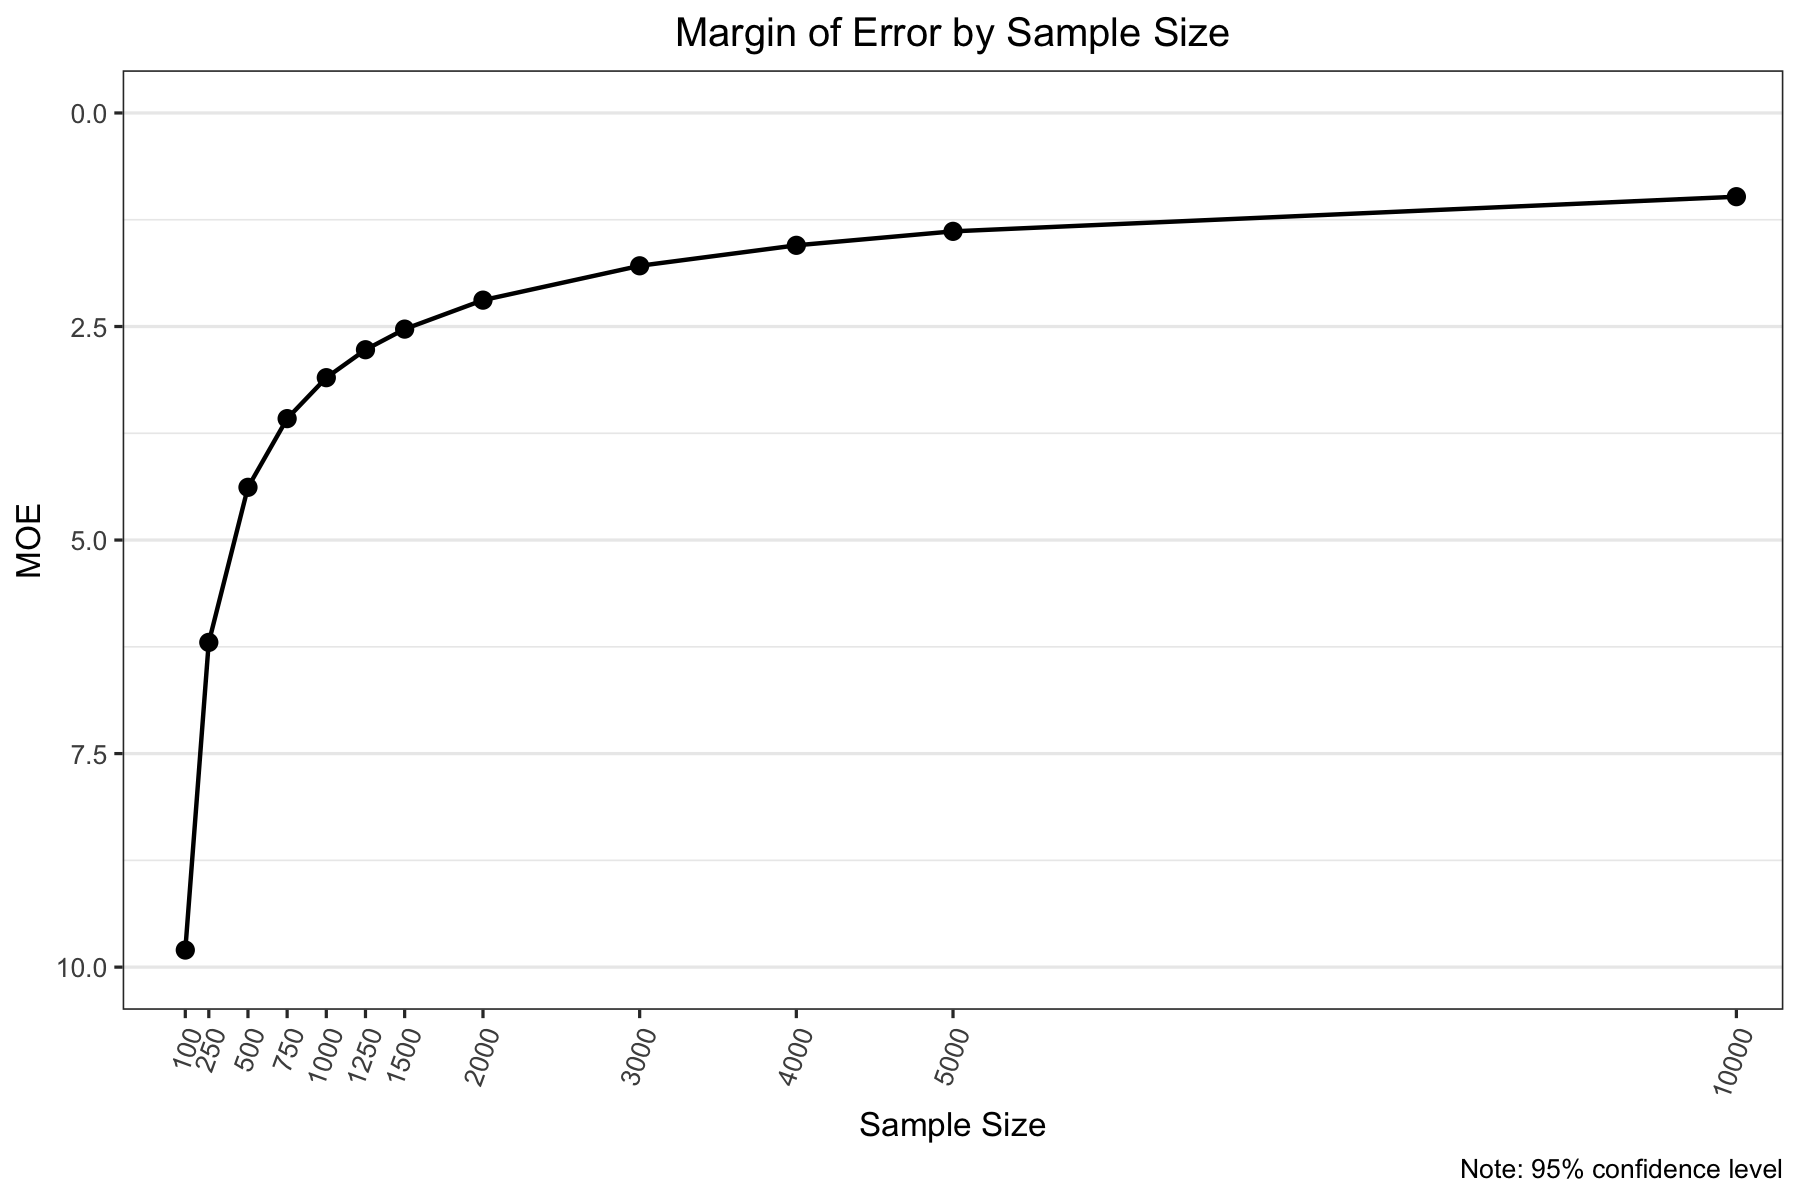
\includegraphics[width=.9\textwidth]{moe_samplesize.png}}
\only<6>{
    \begin{center}
    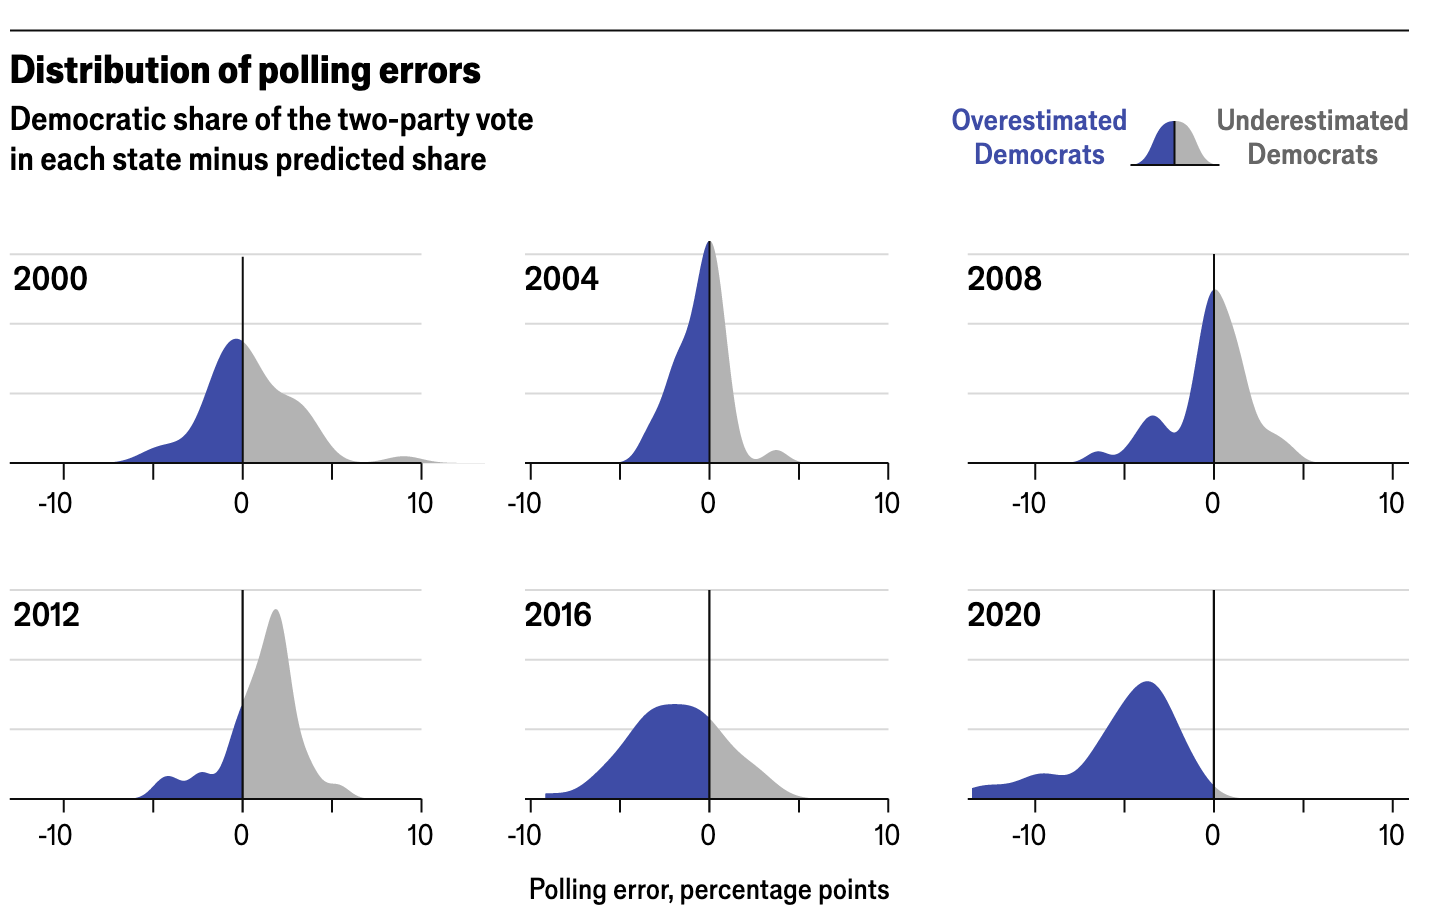
\includegraphics[width=.9\textwidth]{distribution_polling_error.png}
    \end{center}
    {\scriptsize Source: The Economist}
    }
}

%%%%%%%%%%%%%%%%%%%%%%%%%%%%%%%%%%%%%%%%%%%%%%%%%%%%%%%%%%%%%%%%%%
\frame{\frametitle{Getting a Random Sample}
\only<1>{
    \begin{center}
    How would you generate a random sample of American voters?
    \end{center}
}
\only<2->{
    \begin{itemize}[<+(1)->]
        \item \textbf{Systematic Sampling}: Select every $n^{th}$ unit of a population (e.g. exit polls)
        \item \textbf{List-based Sampling}: Randomly select units from an existing list of the population (e.g. registered voter lists)
        \item \textbf{Address-based Sampling (ABS)}: Randomly select households from a list of addresses provided by the U.S. Postal Service
        \item \textbf{Random-digit Dialing (RDD)}: Randomly select area codes, and then random digits are added to the end to create 10-digit phone numbers
        \item \textbf{Non-probability/Quota Sampling}: Pseudo-randomly selecting, from an opt-in pool of respondents, a sample that approximates the make-up of the general population
    \end{itemize}
}
}

\end{document}
